\section{User Study Scenarios and Interfaces}~\label{appx:user}

This appendix summarizes the Wizard-of-Oz user-study materials referenced in Sec.~\ref{exp:user_study}. Each participant completed five waste sorting scenarios and five tomato harvesting scenarios. The mapping between scenarios and interaction conditions was randomized for each participant so that every participant experienced each condition exactly once per domain.

\subsection{Scenario Structure and Questionnaire Timing}~\label{appx:user_scenarios}
Table~\ref{tab:app_user_scenarios} summarizes the scenario identifiers and primary variations used for counterbalancing. The following paragraphs describe the domain-specific scenario structure and post-scenario questionnaires.
The scenario IDs in the table are used only to identify the WoZ materials and randomization records; they do not encode the interaction condition assigned to a participant.

\begin{table}[h]
\centering
\caption{User-study scenario structure. Scenario identifiers were used for counterbalancing and do not imply a fixed condition assignment.}
\label{tab:app_user_scenarios}
\small
\begin{tabular}{lll}
\toprule
\textbf{Domain} & \textbf{Scenario IDs} & \textbf{Primary variation} \\
\midrule
Waste sorting & W1--W5 & Waste category, object order, and detection ambiguity \\
Tomato harvesting & T1--T5 & Tomato state, stem location, and scan/harvest ambiguity \\
\bottomrule
\end{tabular}
\end{table}

\subsubsection{Waste Sorting Scenarios}
The waste sorting trials showed a tabletop scene with four waste objects and category-dependent target bins. Participants answered questions about visually highlighted objects or selected actions depending on the assigned condition. In state-level query conditions, the interface asked participants to verify observable task facts such as whether the highlighted object belonged to a specific waste category. In the \textbf{KnowNo} condition, participants selected the robot's next action, which could require deciding whether the robot should inspect an object again or proceed to grasp and place it.

\subsubsection{Tomato Harvesting Scenarios}
The tomato harvesting trials showed tomatoes attached to two stems and required participants to reason about whether tomatoes should be harvested, ignored, scanned, placed, or discarded. State-level query conditions asked participants to verify facts such as object existence or tomato condition. In \textbf{KnowNo}, participants selected action-level alternatives in the harvesting sequence. These action choices were generally more constrained than in waste sorting because the tomato workflow follows a clearer navigation--detection--pick--scan--place/discard order.

Fig.~\ref{fig:app_user_interface_examples} shows representative interface screens from the user study. The examples include a state-level query interface and action-level KnowNo interfaces to show the difference between verifying a task fact and selecting the next robot action.

\begin{figure*}[t]
    \centering
    \begin{subfigure}[t]{0.32\textwidth}
        \centering
        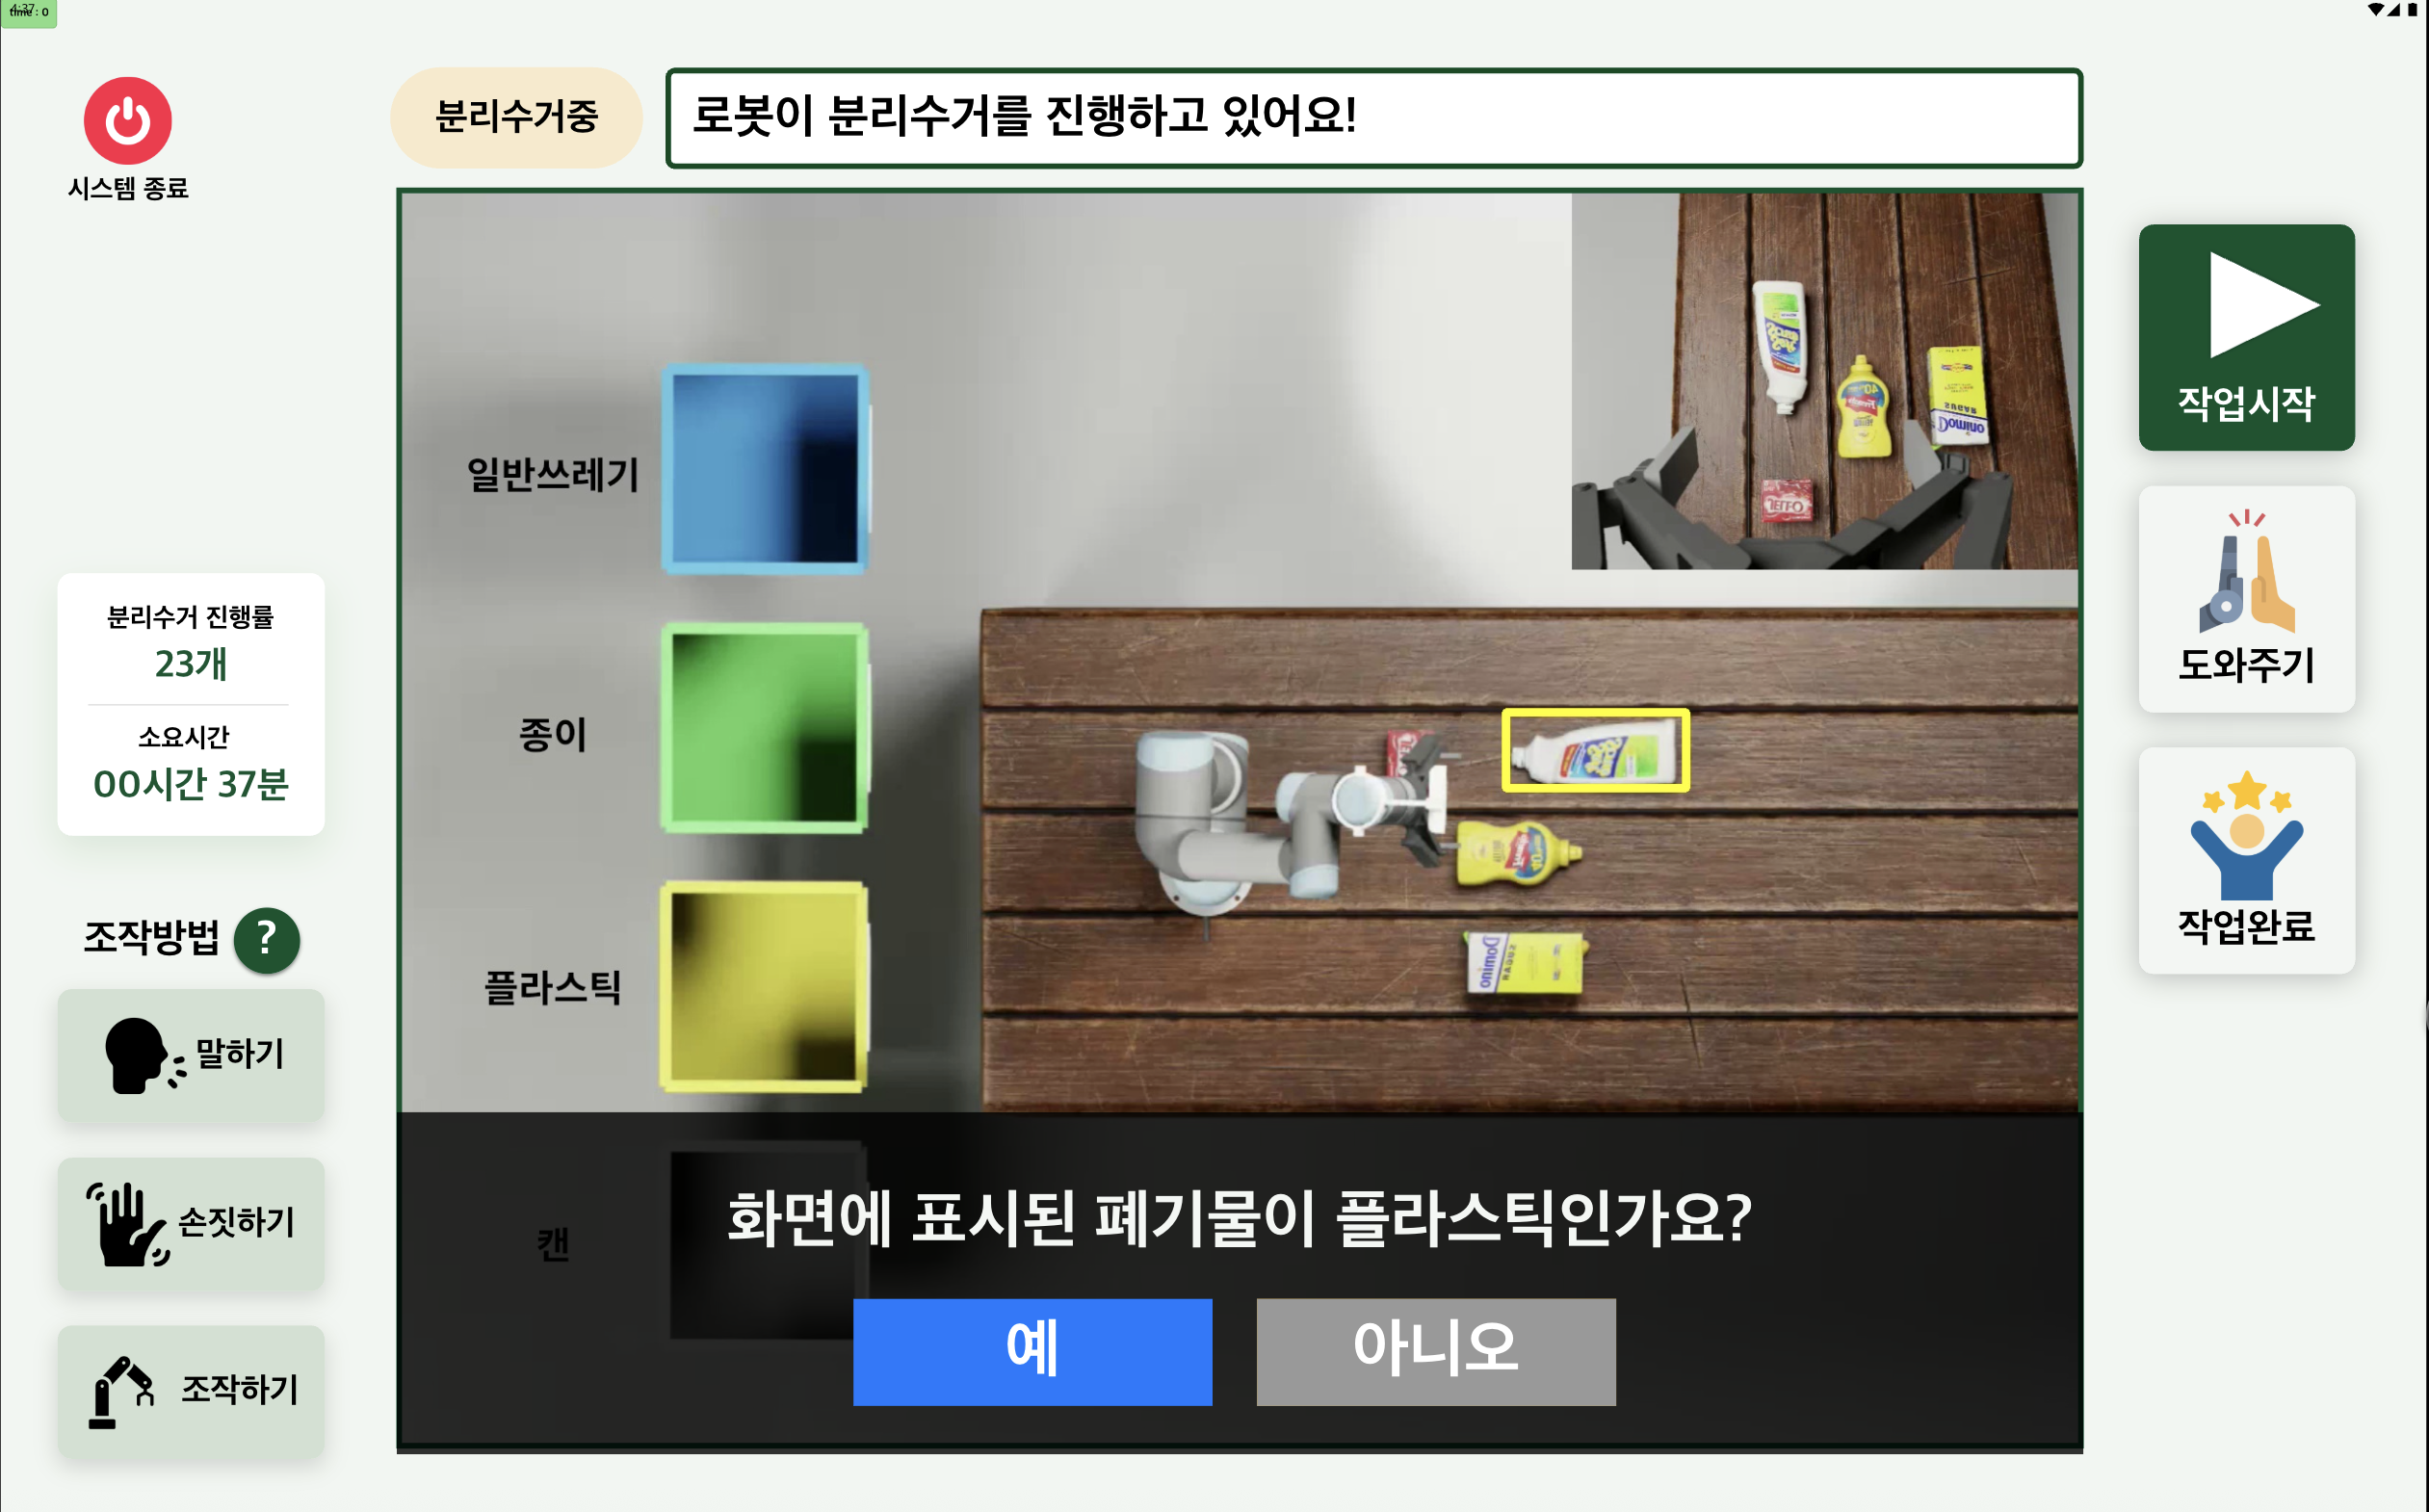
\includegraphics[width=\linewidth]{figures/user_study/fig_waste_our1.png}
        \caption{\textbf{Ours1} in waste sorting.}
        \label{fig:app_user_interface_waste_ours1}
    \end{subfigure}
    \hfill
    \begin{subfigure}[t]{0.32\textwidth}
        \centering
        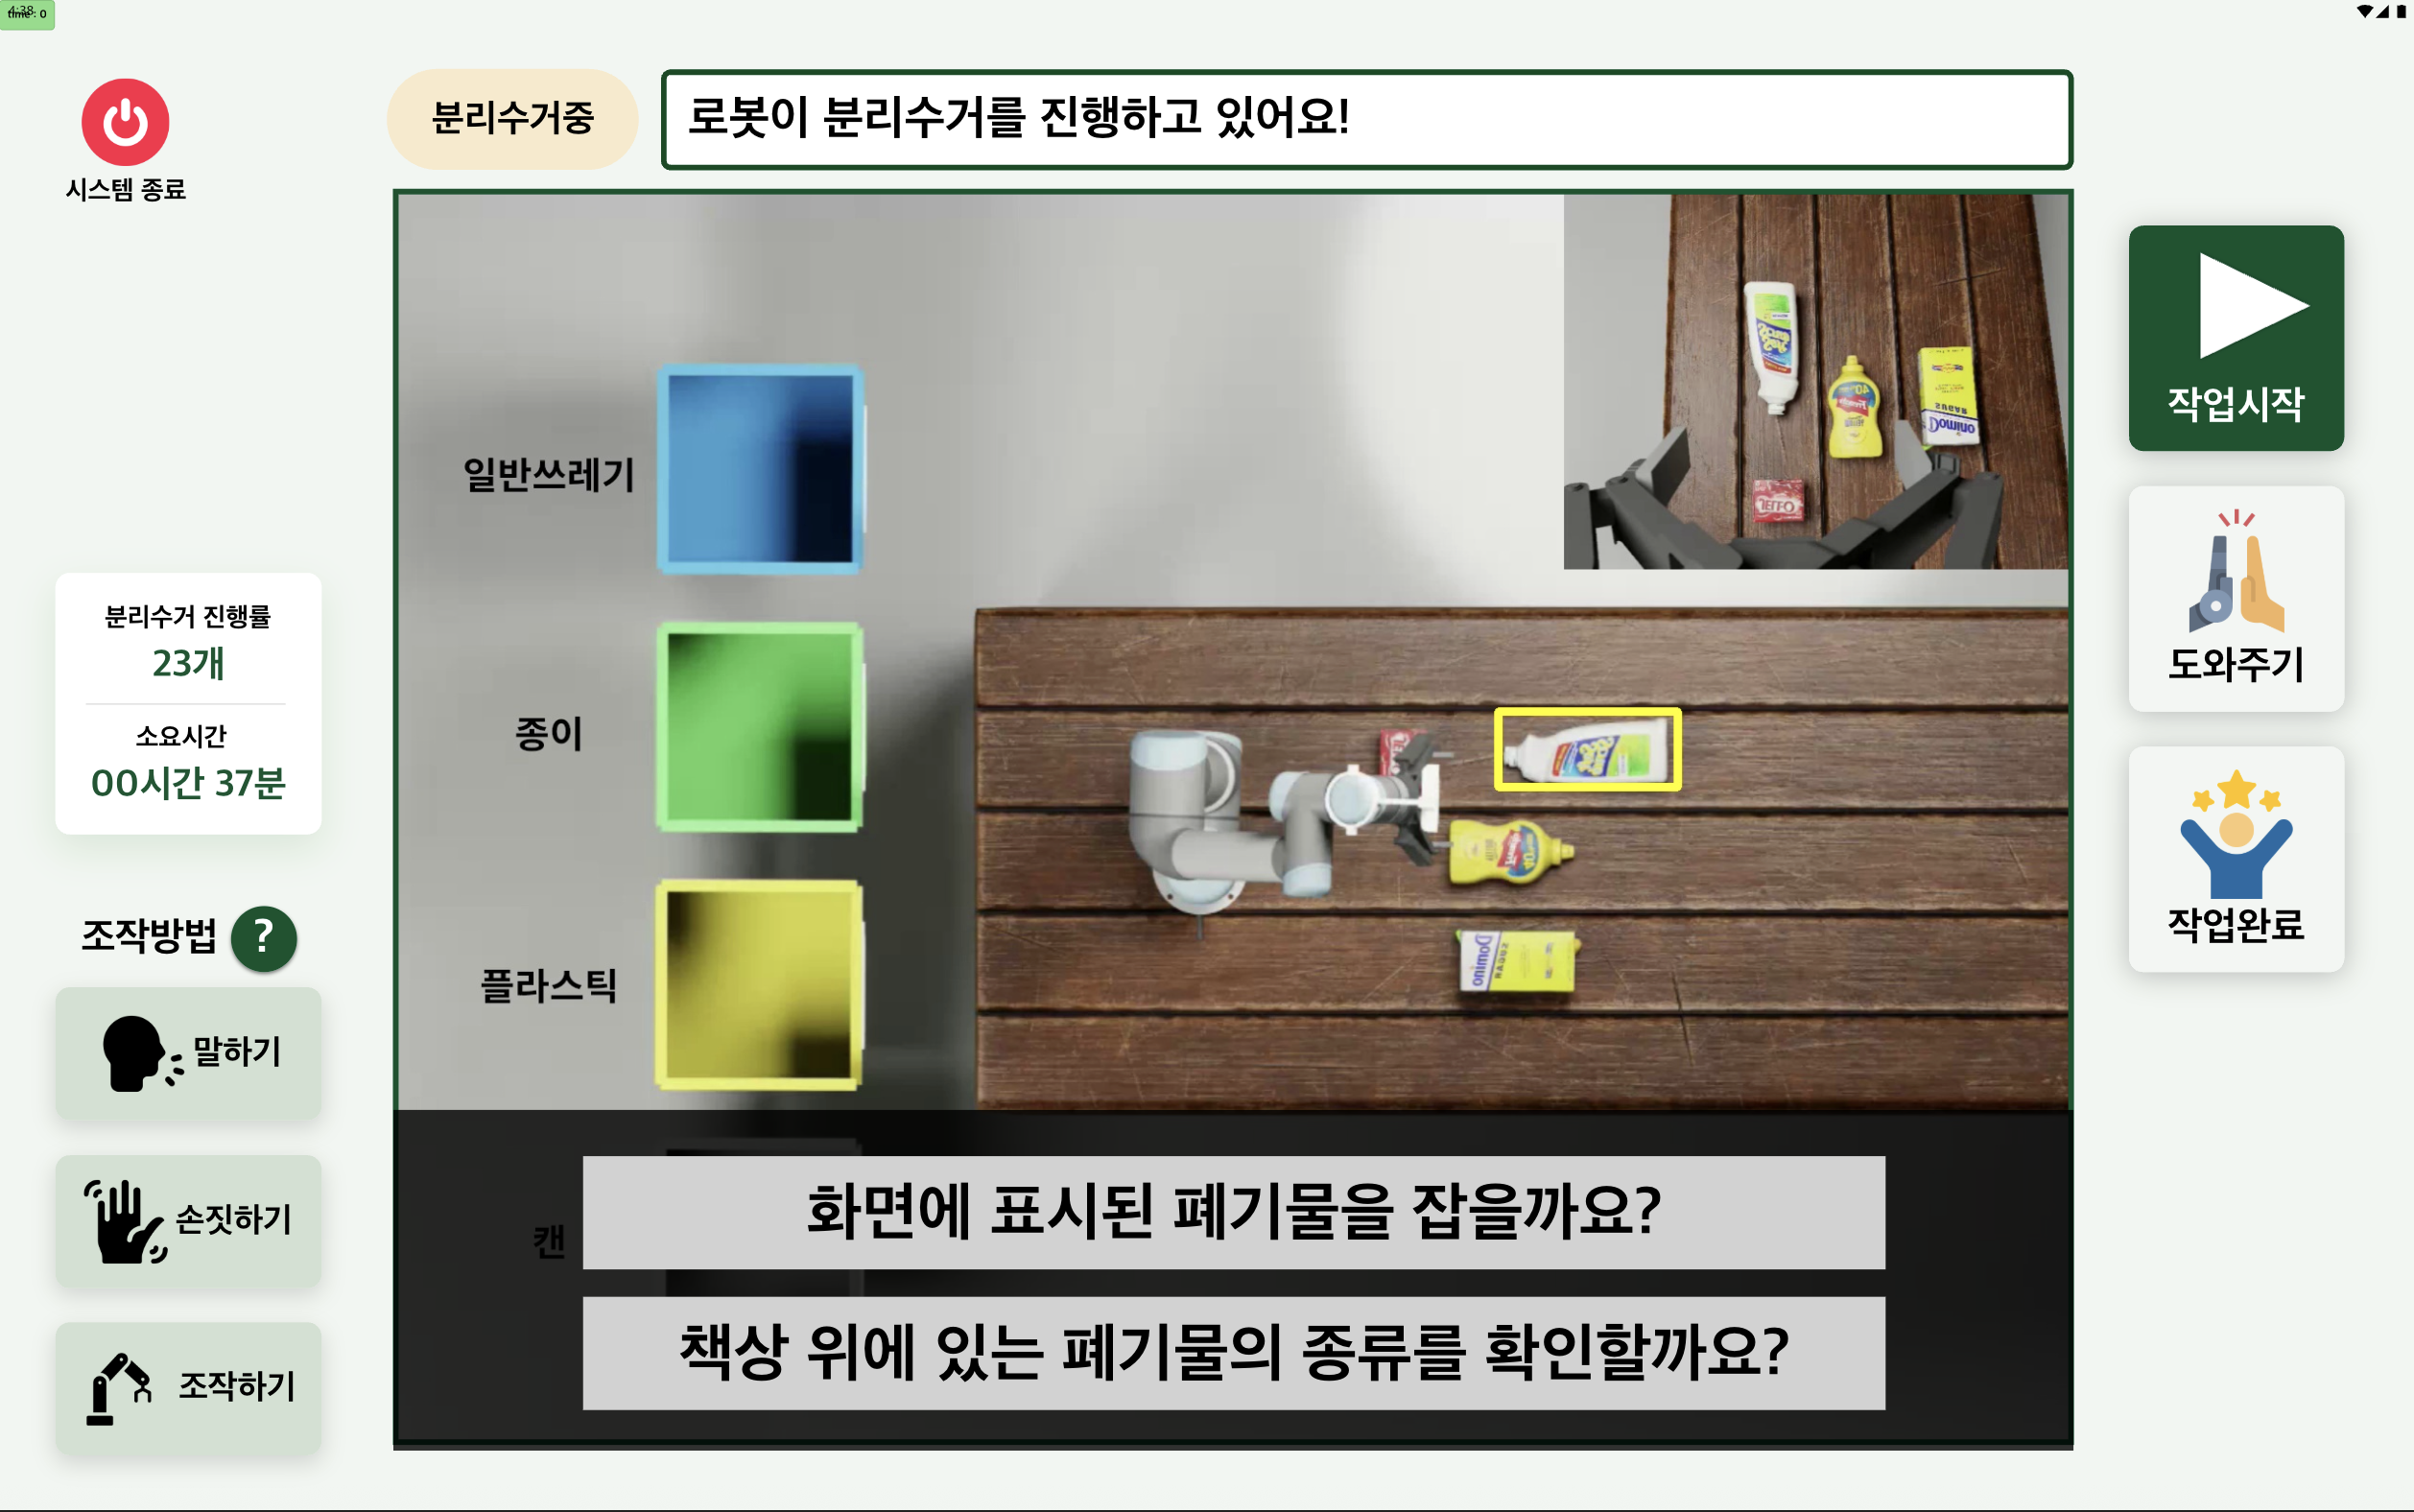
\includegraphics[width=\linewidth]{figures/user_study/fig_waste_knowno.png}
        \caption{\textbf{KnowNo} in waste sorting.}
        \label{fig:app_user_interface_waste_knowno}
    \end{subfigure}
    \hfill
    \begin{subfigure}[t]{0.32\textwidth}
        \centering
        
\includegraphics[width=\linewidth]{figures/user_study/fig_tomato_knowno.png}
        \caption{\textbf{KnowNo} in tomato harvesting.}
        \label{fig:app_user_interface_tomato_knowno}
    \end{subfigure}
    \caption{Representative user-study interfaces. The proposed state-query interface asks users to verify observable task facts, whereas the action-query baseline asks users to choose the next robot action.}
    \label{fig:app_user_interface_examples}
\end{figure*}

\subsubsection{Questionnaire Timing}
After each scenario, participants completed NASA Raw-TLX, fatigue, SART, and SAGAT-style items. SAGAT questions were grouped into three levels: Lv1 for perception of the current state, Lv2 for comprehension of the task situation, and Lv3 for projection of future robot behavior. The analyses in Sec.~\ref{user:results_workload_sa} and Sec.~\ref{user:results_sagat_levels} use these post-scenario responses.

\subsection{Condition Codes and Participant-Level Assignment}~\label{appx:user_assignment}

Table~\ref{tab:app_condition_codes} defines the condition codes used in the user-study logs. Table~\ref{tab:app_participant_condition_order} reports the participant-level trial order reconstructed from the survey timestamps. Each token has the form \texttt{D\_SxCy}, where \texttt{D} is the domain (\texttt{W}: waste sorting, \texttt{T}: tomato harvesting), \texttt{Sx} is the scenario identifier, and \texttt{Cy} is the condition code. Participants completed the two domain blocks in different orders, so the table is split into the first five and last five trials rather than assuming that tomato harvesting always preceded waste sorting.
The condition-code table is used to decode the compact trial-order tokens and the scenario-level answer summaries below.

\begin{table}[h]
\centering
\caption{Condition-code definitions used in the user-study logs.}
\label{tab:app_condition_codes}
\small
\begin{tabular}{cll}
\toprule
\textbf{Code} & \textbf{Condition} & \textbf{Interaction policy} \\
\midrule
C1 & All & Query whenever feedback is available \\
C2 & No & No user feedback request \\
C3 & Ours1 & State-level uncertainty query policy \\
C4 & Ours2 & State-level query exposure condition with varied transition profile \\
C5 & KnowNo & Action-level query baseline \\
\bottomrule
\end{tabular}
\end{table}

\begin{table*}[t]
\centering
\caption{Participant-level condition assignment and timestamp-reconstructed trial order.}
\label{tab:app_participant_condition_order}
\scriptsize
\setlength{\tabcolsep}{3pt}
\begin{tabular*}{\textwidth}{@{\extracolsep{\fill}}lll}
\toprule
\textbf{Participant} & \textbf{Trials 1--5} & \textbf{Trials 6--10} \\
\midrule
p001 & T\_S1C1, T\_S4C4, T\_S4C5, T\_S2C3, T\_S3C2 & W\_S4C5, W\_S1C2, W\_S5C1, W\_S2C3, W\_S3C4 \\
p002 & T\_S4C5, T\_S2C3, T\_S1C1, T\_S3C2, T\_S5C4 & W\_S3C2, W\_S4C3, W\_S1C5, W\_S2C4, W\_S5C1 \\
p003 & W\_S4C4, W\_S3C5, W\_S1C1, W\_S5C3, W\_S2C2 & T\_S4C3, T\_S2C1, T\_S1C2, T\_S5C4, T\_S3C5 \\
p004 & W\_S3C2, W\_S4C1, W\_S2C4, W\_S5C3, W\_S1C5 & T\_S5C1, T\_S2C2, T\_S1C3, T\_S3C5, T\_S4C4 \\
p005 & W\_S1C2, W\_S4C5, W\_S2C4, W\_S3C1, W\_S5C3 & T\_S2C2, T\_S5C4, T\_S4C1, T\_S3C3, T\_S1C5 \\
p006 & T\_S5C2, T\_S2C4, T\_S3C5, T\_S1C1, T\_S4C3 & W\_S2C2, W\_S3C3, W\_S5C5, W\_S1C4, W\_S4C1 \\
p007 & T\_S3C1, T\_S5C4, T\_S2C5, T\_S1C2, T\_S4C3 & W\_S4C5, W\_S1C3, W\_S2C4, W\_S3C1, W\_S5C2 \\
p008 & W\_S3C1, W\_S1C4, W\_S4C3, W\_S2C5, W\_S5C2 & T\_S1C5, T\_S5C2, T\_S4C1, T\_S2C3, T\_S3C4 \\
p009 & W\_S3C4, W\_S5C2, W\_S1C1, W\_S4C5, W\_S2C3 & T\_S4C1, T\_S5C3, T\_S2C5, T\_S1C4, T\_S3C2 \\
p010 & W\_S4C4, W\_S2C2, W\_S5C5, W\_S1C1, W\_S4C3 & T\_S2C1, T\_S1C5, T\_S5C3, T\_S4C4, T\_S3C2 \\
p011 & W\_S2C2, W\_S3C3, W\_S1C1, W\_S2C4, W\_S4C5 & T\_S2C1, T\_S1C5, T\_S5C2, T\_S4C4, T\_S3C3 \\
p012 & W\_S3C3, W\_S5C5, W\_S4C4, W\_S1C1, W\_S2C2 & T\_S4C2, T\_S3C3, T\_S2C5, T\_S5C4, T\_S1C1 \\
\bottomrule
\end{tabular*}
\end{table*}

\subsection{Questionnaires}~\label{appx:user_questionnaires}

The questionnaires were administered in Korean. The following English translation lists the questionnaire content used in the user study.
Tables~\ref{tab:app_sagat_tomato_questions} and~\ref{tab:app_sagat_waste_questions} list the SAGAT-style items used after tomato-harvesting and waste-sorting scenarios, respectively. The item levels correspond to the Lv1--Lv3 situation-awareness categories reported in Sec.~\ref{user:results_sagat_levels}. Table~\ref{tab:app_workload_sart_questions} lists the post-scenario workload, fatigue, and SART items administered after each trial.

\begin{table*}[t]
\centering
\caption{SAGAT-style questionnaire items for tomato harvesting.}
\label{tab:app_sagat_tomato_questions}
\scriptsize
\setlength{\tabcolsep}{3pt}
\begin{tabularx}{\textwidth}{p{0.05\textwidth}p{0.09\textwidth}p{0.40\textwidth}X}
\toprule
\textbf{Item} & \textbf{Level} & \textbf{Question} & \textbf{Options} \\
\midrule
Q1 & Lv1 & How many tomatoes are currently displayed on the screen? & 0; 1; 2; I do not know \\
Q2 & Lv1 & What was the state of the tomato most recently processed by the robot? & Ripe; unripe; damaged/rotten; I do not know \\
Q3 & Lv2 & What is the key information that the user should judge in the current situation? & Whether the target tomato is harvestable; whether the robot should move to the next location; whether there is information that the robot judged incorrectly; I do not know \\
Q4 & Lv2 & Why is user confirmation needed in the current situation? & Tomato ripeness judgment is uncertain; tomato damage judgment is uncertain; a harvest target may have been missed; I do not know \\
Q5 & Lv3 & If the user takes no action, what is the robot most likely to do? & Remain waiting; continue the task according to the current judgment; terminate the task; I do not know \\
Q6 & Lv3 & If the robot selected the wrong tomato and the user does not correct it, what is the most likely outcome? & The wrong tomato may be harvested; the robot will automatically select the correct tomato again; the task will terminate immediately; I do not know \\
\bottomrule
\end{tabularx}
\end{table*}

\begin{table*}[t]
\centering
\caption{SAGAT-style questionnaire items for waste sorting.}
\label{tab:app_sagat_waste_questions}
\scriptsize
\setlength{\tabcolsep}{3pt}
\begin{tabularx}{\textwidth}{p{0.05\textwidth}p{0.09\textwidth}p{0.40\textwidth}X}
\toprule
\textbf{Item} & \textbf{Level} & \textbf{Question} & \textbf{Options} \\
\midrule
Q1 & Lv1 & How many objects are currently on the table in the screen? & 0; 1; 2 or more; I do not know \\
Q2 & Lv1 & What was the material/category of the waste object most recently processed by the robot? & Plastic; can; general waste; paper \\
Q3 & Lv2 & What is the key information that the user should judge in the current situation? & Whether the next object exists; whether the target object can be grasped from the current position; whether the target object was moved to the correct recycling bin; I do not know \\
Q4 & Lv2 & Why was user confirmation needed in the previous situation? & Target object's waste category judgment is uncertain; target object is outside the robot's reachable range; target object is contaminated and its recyclability should be judged; I do not know \\
Q5 & Lv3 & If the user takes no action, what is the robot most likely to do? & Remain waiting; continue the waste-sorting task according to the current judgment; terminate the task; I do not know \\
Q6 & Lv3 & If the robot sorted an object incorrectly and the user does not correct the task, what is the most likely outcome? & Target object may be placed in the wrong bin; the robot will automatically recognize the error and sort it again; the robot will immediately terminate all waste sorting; I do not know \\
\bottomrule
\end{tabularx}
\end{table*}

\begin{table*}[t]
\centering
\caption{Post-scenario workload, fatigue, and situation-awareness questionnaire items.}
\label{tab:app_workload_sart_questions}
\scriptsize
\setlength{\tabcolsep}{4pt}
\begin{tabularx}{\textwidth}{p{0.08\textwidth}p{0.17\textwidth}X}
\toprule
\textbf{Item} & \textbf{Measure} & \textbf{Question} \\
\midrule
N1 & NASA Raw-TLX & How mentally demanding was this task? \\
N2 & NASA Raw-TLX & How physically demanding was this task? \\
N3 & NASA Raw-TLX & How hurried or rushed did the task pace feel? \\
N4 & NASA Raw-TLX & How successful did you feel in performing the requested task? \\
N5 & NASA Raw-TLX & How hard did you have to work to achieve task success? \\
N6 & NASA Raw-TLX & How insecure, discouraged, irritated, stressed, or annoyed did you feel during the task? \\
F & Cognitive fatigue & What was your level of fatigue? \\
S1 & SART & How unstable or changeable was the situation? \\
S2 & SART & How complicated was the situation? \\
S3 & SART & How many variables were changing within the situation? \\
S4 & SART & How alert were you in the current situation? \\
S5 & SART & How focused were you on the current situation? \\
S6 & SART & How divided was your attention in the current situation? \\
S7 & SART & How much spare cognitive capacity did you have in the current situation? \\
S8 & SART & How much information did you obtain about the current situation? \\
S9 & SART & How good was the information you obtained about the current situation? \\
S10 & SART & How familiar were you with the current situation? \\
\bottomrule
\end{tabularx}
\end{table*}

\subsection{Scenario-Level Answer Summary}~\label{appx:user_answer_summary}

Table~\ref{tab:app_answer_summary} summarizes the scenario-condition scoring records used for task-response correctness. The columns report the number of scored trials, the mean number of correct responses over the mean number of scorable responses, and the corresponding mean accuracy. Condition codes follow Table~\ref{tab:app_condition_codes}. The \textbf{No} condition (C2) is omitted from this summary because it did not request user responses and therefore did not produce scorable task answers.

\begin{table*}[t]
\centering
\caption{Scenario-condition answer summaries for tomato harvesting and waste sorting.}
\label{tab:app_answer_summary}
\begin{minipage}[t]{0.48\textwidth}
\centering
\textbf{Tomato harvesting}
\vspace{2pt}

\scriptsize
\setlength{\tabcolsep}{0pt}
\begin{tabular*}{\linewidth}{@{\extracolsep{\fill}}llccc}
\toprule
\textbf{Scen.} & \textbf{Cond.} & \textbf{$n$} & \textbf{Correct/Total} & \textbf{Acc.} \\
\midrule
S1 & C1 & 4 & 13.0/13.8 & 0.95 \\
S1 & C3 & 1 & 8.0/8.0 & 1.00 \\
S1 & C4 & 1 & 7.0/7.0 & 1.00 \\
S1 & C5 & 4 & 4.0/4.0 & 1.00 \\
S2 & C1 & 3 & 13.7/14.0 & 0.98 \\
S2 & C3 & 3 & 6.3/7.0 & 0.90 \\
S2 & C4 & 1 & 7.0/7.0 & 1.00 \\
S2 & C5 & 3 & 4.0/4.0 & 1.00 \\
S3 & C1 & 1 & 14.0/14.0 & 1.00 \\
S3 & C3 & 3 & 6.7/7.0 & 0.95 \\
S3 & C4 & 1 & 6.0/6.0 & 1.00 \\
S3 & C5 & 3 & 3.0/3.0 & 1.00 \\
S4 & C1 & 3 & 13.3/13.7 & 0.98 \\
S4 & C3 & 3 & 7.3/8.0 & 0.92 \\
S4 & C4 & 4 & 6.8/7.0 & 0.96 \\
S4 & C5 & 1 & 4.0/4.0 & 1.00 \\
S5 & C1 & 1 & 11.0/13.0 & 0.85 \\
S5 & C3 & 2 & 7.0/7.0 & 1.00 \\
S5 & C4 & 5 & 5.6/6.0 & 0.93 \\
S5 & C5 & 1 & 2.0/3.0 & 0.67 \\
\bottomrule
\end{tabular*}
\end{minipage}
\hfill
\begin{minipage}[t]{0.48\textwidth}
\centering
\textbf{Waste sorting}
\vspace{2pt}

\scriptsize
\setlength{\tabcolsep}{0pt}
\begin{tabular*}{\linewidth}{@{\extracolsep{\fill}}llccc}
\toprule
\textbf{Scen.} & \textbf{Cond.} & \textbf{$n$} & \textbf{Correct/Total} & \textbf{Acc.} \\
\midrule
S1 & C1 & 5 & 11.8/12.0 & 0.98 \\
S1 & C3 & 1 & 5.0/5.0 & 1.00 \\
S1 & C4 & 2 & 6.0/6.0 & 1.00 \\
S1 & C5 & 2 & 2.0/3.0 & 0.67 \\
S2 & C3 & 2 & 5.0/5.0 & 1.00 \\
S2 & C4 & 5 & 5.0/5.0 & 1.00 \\
S2 & C5 & 1 & 2.0/3.0 & 0.67 \\
S3 & C1 & 3 & 12.3/12.3 & 1.00 \\
S3 & C3 & 3 & 5.0/5.0 & 1.00 \\
S3 & C4 & 2 & 5.0/5.0 & 1.00 \\
S3 & C5 & 1 & 3.0/3.0 & 1.00 \\
S4 & C1 & 2 & 12.0/12.0 & 1.00 \\
S4 & C3 & 3 & 4.3/5.0 & 0.87 \\
S4 & C4 & 3 & 4.0/4.0 & 1.00 \\
S4 & C5 & 5 & 2.4/4.0 & 0.60 \\
S5 & C1 & 2 & 11.5/12.0 & 0.96 \\
S5 & C3 & 3 & 5.0/5.0 & 1.00 \\
S5 & C5 & 3 & 3.0/4.0 & 0.75 \\
\bottomrule
\end{tabular*}
\end{minipage}
\end{table*}
